\chapter{LRDE Presentation}


\section{Line of business}
The \LRDE\space (Research and Development Laboratory of \EPITA) is focused on fundamental
research and development in computer science. Its main areas of expertise are:
\begin{itemize}
 \item Image processing and pattern recognition
 \item Automata and verification
 \item Performance and genericity
\end{itemize}


\noindent Building on its solid scientific production and academic collaborations, the laboratory has
industrial contracts, conducts internal research projects and participates in collaborative
academic research projects.

\noindent Its members also give classes to students at \EPITA\space from the first year of engineering.

\section{The Laboratory}
The \LRDE\space (\url{https://www.lrde.epita.fr/wiki/Home}) was created in February 1998 to promote
the research activity at \EPITA\space and to allow students to be involved into important research
projects.

The research activity at \LRDE\space is focusing on subjects related to the school with the aim
of getting recognition in the scientific domain through publications and by working together with other
research centers.\\
One particularity of the \LRDE\space is the will to create a bond between traditional
teaching given to \EPITA\space students and teaching through research. The point of this is to:
\begin{itemize}
  \item participate to the production of knowledge in computer science and to
	promote the image of \EPITA\space in scientific domain.
  \item develop \LRDE\space student's formation through research and allow them to access a third cycle
	formation.
\end{itemize}


\section{Members}
The laboratory is currently composed of thirteen permanent members, including teacher-researchers, engineers
and administration.

\noindent In addition to permanent staff, the \LRDE\space also hosts PhD students. Currently, there are five of them.
During the whole duration of their doctoral studies, they work with two advisor researchers, one of the
\LRDE\space and one of another university (joint supervision in partnership).

Each year, the permanent members recruit third year students from \EPITA, whom will stay until the
end of their studies, following a dedicated study specialisation at \EPITA\space. Hence, the laboratory
hosts two generations of students that can grow to a number between ten to fifteen.


\section{Services}
The \LRDE\space is working on four different axis:


\subsection{Image Processing}
\subsubsection{Olena}
\begin{center}
 
\includegraphics[width=2cm]{img/olena.jpg}
\end{center}
The Olena project (\url{https://olena.lrde.epita.fr}) consists of a generic image processing library.
Its objective is to implement a platform of numerical scientific computations dedicated to image
processing, pattern recognition and computer vision. This environment is composed of a generic and
efficient library (Milena), a set of tools for shell scripts and a visual programming interface.
The project aims at offering an interpreted environment like MatLab or Mathematica. It provides many
ready-to-use image data structures (regular 1D, 2D, 3D images, graph-based images, etc.) and algorithms.
Milena's algorithms are built upon classical entities from the image processing field (images, points/sites,
domains, neighborhoods, etc.).\\

Each of these parts imply its own difficulties and require the development of new solutions.
For example, the library, which require the entirety of low level features on which it relies on to be
both efficient and generic --- two objectives that are hard to meet at the same time in programmation.
Fortunately, the object oriented programming eases this problem if we avoid the classical object
modeling with inheritance and polymorphism. Hence, this genericity allows the development of efficient
and re-usable code - i.e. developers or practitioners can easily understand, modify, develop and extend
new algorithms while retaining the core traits of Milena: genericity and efficiency.
The Olena platform uses this paradigm. The project already addressed the problem of the diversity of data
and data structures.\\

Furthermore, the people working on this project were able to put in light the existence of conception
models related to generic programmation. Olena is an open source project under General Public License (GPL)
version 2.


\subsubsection{Climb}
The Climb team of the laboratory has chosen to focus on the persistent question of performance and
genericity, only from a different point of view.\\

The purpose of this research is to examine the solutions offered by languages other than C++, dynamic
languages notably, and Lisp in particular. C++ has its drawbacks, it is a heavy language with an extremely
complex and ambiguous syntax, the template system is actually a completely different language from standard
C++ and finally it is a static language. This last point has significant implications on the application,
insofar as it imposes a strict chain of Compilation $\rightarrow$ Development $\rightarrow$ Run
$\rightarrow$ Debug, making for example rapid prototyping or human-machine interfacing activities difficult.
It becomes therefore essential to equip the involved projects with a third language infrastructure that is
rather based on scripting languages.\\

The Climb project aims at investigating the same domain as Olena, but starting from an opposite view.
It express the same issues following an axis of dynamic genericity and compares the performance obtained by
some Common Lisp compilers with those of equivalent programs written in C or C++.

\subsection{Finite state machine manipulation}
\subsubsection{\VCSN}
\begin{center}
 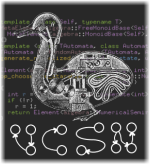
\includegraphics[width=2cm]{img/vcsn.png}
\end{center}
The \VCSN project (\url{https://vcsn.lrde.epita.fr}) is a finite state machine manipulation
platform developed in collaboration with the ENST. Finite state machines, also called automata,
are useful for language treatment and task automation. In the past, such platforms, like "FSM",
were supposed to work for problems of industrial scale. Hence, for efficiency reasons, they were
specialized in letter automata. On the other hand, platforms like "FSA" were based on a more abstract
approach. \VCSN tries to answer both of these issues by using techniques of static and generic
programmation in C++.\\

\VCSN can then support the entirety of automata with multiplicity in any kind of
semiring. Thanks to generic programming techniques, it is not necessary to code a single algorithm once
for each type of automata anymore. A single abstract version is sufficient, and this without loosing
efficiency. It is not necessary to handle C++ perfectly to be able to use the platform thanks to an
interpreter conceived to highlight all of the system's potential. This environment should allow
researchers to experiment their ideas and beginners to practice with an intuitive interface.\\

\VCSN is an open source project under GPL license.


\subsection{Model checking}
\subsubsection{Spot}
\begin{center}
 
\includegraphics[width=2cm]{img/spot.png}
\end{center}
Spot (\url{https://spot.lrde.epita.fr/}) is a library of algorithms for "model checking",
which is a way to check that every possible behavior of a system satisy its given properties.
Spot allows to express those properties using linear-time temporal logic (LTL). It corresponds to classical
propositional calculus (with its "or", "and" and "not" operators) equiped with temporal operators to
express things such as "in a future time" or "anytime since now". Spot also supports arbitrary 
acceptance condition, transition-based acceptance and four different representation formats of
$\omega$-automata (HOA, never claims, LBTT, DSTAR). All those terms will be explained in the 'basic
concepts' section.\\

Such formulas seen above (LTL formulas) can be translated to automata (Spot implements different algorithms)
, such that verifying that the behavior of a model satisfy a formula can be reduced to operations between
two automata (here again Spot implements different algorithms). This approach can be applied to different kind of systems: communication protocoles,
electronic circuits, programs...\\

This project was born in the MoVe team at LIP6, but since 2007 it is mainly developped by the LRDE, with some
occasional collaborations with LIP6. It is distributed under a GNU GPL version 3 license. 


\subsection{Speaker recognition}
\subsubsection{Speaker ID}
The Speaker Recognition team is working on Machine Learning solutions applied to Speaker Recognition
tasks. They propose statistical representations of speech signal which are more robust to the problem
of session and channel variabilities.\\

A speaker must always be identified, whether he is ill, suffering from sore throats, or his
current emotions bring change to his voice. To do this, all the characteristics of a voice that can change
depending on any external parameter must be ignored. This is one of the issues the Speaker ID team is
facing.\\

They participated in the evaluation campaign of speaker verification systems organized by NIST
(the National Institute of Standards and Technology) which organizes competitions in various fields, both
to stimulate research and to define new standards since the beginning of the project.\\

The work of LRDE Speaker ID team is conducted in collaboration with the Spoken Language Systems Group of
the MIT Computer Science and Artificial Intelligence Laboratory (\url{http://groups.csail.mit.edu/sls/}).


\section{The internship in the company's work}
This internship took place within the team of model checking. It was essentially focused on
the improvement of the SAT-based minimization of $\omega$-automata. It covers one of the many
features of the Spot library.